\chapter{Desarrollo vegetativo de las plantas: meristemos y crecimiento}\label{ch:b2:plant-meristems}

Un roble que era una plántula cuando se construyó la catedral sigue
añadiendo cada año un anillo de \omterm{def:b2:plant-meristems:wood}{madera}, sigue abriendo hojas nuevas cada
primavera, sigue abriendo paso a nuevos ápices radiculares a través del
suelo. Ningún animal hace esto; un caballo deja de crecer a los cuatro
años. La diferencia es que una planta conserva, en el extremo de cada
tallo y de cada raíz y en un fino cilindro dentro de cada tronco, pequeñas
poblaciones de células embrionarias --- los \emph{\omterm{def:b2:plant-meristems:meristem}{meristemos}} --- que
nunca dejan de dividirse y que construyen el cuerpo de la planta hacia
fuera y hacia arriba mientras vive. Este capítulo examina cómo están
organizados y controlados los dos \omterm{def:b2:plant-meristems:meristem}{meristemos} apicales, cómo crece una
célula vegetal, cómo deciden las hormonas la forma de un tallo y cómo se
engrosa un tronco.

\section{Los meristemos}

\begin{definition}[Los meristemos y los dos tipos de crecimiento]\label{def:b2:plant-meristems:meristem}
\index{meristemo}\index{meristemo apical caulinar}\index{meristemo apical radicular}\index{cámbium}
Un \emph{meristemo} es una población de células pequeñas, no
diferenciadas y en división, que persiste durante toda la vida de la
planta y de la que derivan todos sus tejidos. El \emph{meristemo apical
caulinar} (SAM), en el extremo de cada tallo, forma hojas, tallo y, en su
estación, \omterm{def:b2:angiosperm-reproduction:flower}{flores}; el \emph{meristemo apical radicular} (RAM), detrás de
cada ápice radicular, forma la raíz; juntos impulsan el
\emph{crecimiento primario}, el alargamiento de la planta. Los
\emph{meristemos laterales} --- el \emph{\omterm{def:b2:plant-meristems:wood}{cámbium vascular}} y el
\emph{felógeno}, finos cilindros dentro de tallos y raíces --- impulsan el
\emph{crecimiento secundario}, el engrosamiento que forma la \omterm{def:b2:plant-meristems:wood}{madera} y la
\omterm{def:b2:plant-meristems:wood}{corteza}. El crecimiento vegetal es, por tanto, \emph{indefinido}: los
meristemos pueden seguir funcionando indefinidamente, y la planta es un
organismo modular que repite la unidad hoja--nudo--entrenudo--yema
mientras las condiciones lo permitan. Cada yema axilar es un SAM latente,
de modo que una planta lleva miles de puntos de crecimiento de reserva.
\end{definition}

\begin{proposition}[El ápice caulinar]\label{prop:b2:plant-meristems:sam}
\index{filotaxis}\index{primordio foliar}\index{plastocrono}
El SAM es una cúpula de una décima de milímetro de diámetro, formada por
unos pocos cientos de células. Sus una o dos capas externas (la
\emph{túnica}) solo se dividen en el plano de la superficie y dan la
epidermis; la masa situada debajo (el \emph{cuerpo}) se divide en todos
los planos. En la cima, una \emph{zona central} de \omterm{def:b2:cell-differentiation:differentiation}{células madre} que se
dividen lentamente abastece a una \emph{zona periférica} de células que se
dividen más deprisa, donde los \emph{\omterm{prop:b2:plant-meristems:sam}{primordios foliares}} surgen como
abultamientos a intervalos regulares de tiempo (el \emph{plastocrono}, de
horas a días) y a ángulos regulares alrededor de la cúpula (la
\emph{filotaxis}: opuesta, verticilada o en espiral según el ángulo áureo
de \qty{137.5}{\degree}, que coloca cada hoja nueva en el mayor hueco que
dejan las demás). Debajo, una \emph{zona medular} forma la médula y alarga
el tallo. Un primordio se forma donde la hormona auxina se acumula en la
capa superficial y, al crecer, drena la auxina de su entorno, y por eso el
primordio siguiente surge lo más lejos posible de él: el patrón se
autoorganiza.
\end{proposition}

\begin{omfigure}
\begin{tikzpicture}[every node/.style={font=\scriptsize}]
  % dome
  \draw[thick, fill=omExo!12] (-2.2,0) .. controls (-2.2,1.6) and (-0.8,2.6) .. (0,2.6) .. controls (0.8,2.6) and (2.2,1.6) .. (2.2,0) -- (2.2,-1.4) -- (-2.2,-1.4) -- cycle;
  % tunica layers
  \draw[thick, omDef] (-2.2,0) .. controls (-2.2,1.5) and (-0.8,2.45) .. (0,2.45) .. controls (0.8,2.45) and (2.2,1.5) .. (2.2,0);
  \draw[thick, omDef] (-2.05,0) .. controls (-2.05,1.35) and (-0.75,2.3) .. (0,2.3) .. controls (0.75,2.3) and (2.05,1.35) .. (2.05,0);
  % zones
  \draw[thick, dashed, omThm, fill=omThm!15] (0,1.75) ellipse (0.6 and 0.55);
  \draw[thick, dashed, omProp] (0,0.9) ellipse (1.6 and 1.35);
  \draw[thick, dashed, omExo!70!black] (-0.9,-0.9) rectangle (0.9,-0.1);
  % primordia
  \draw[thick, fill=omExo!40] (-2.2,0.4) .. controls (-2.5,1.4) and (-1.6,1.9) .. (-1.55,1.3) .. controls (-1.5,0.9) and (-1.9,0.6) .. (-2.2,0.4);
  \draw[thick, fill=omExo!40] (2.2,0.2) .. controls (2.7,1.0) and (2.1,1.5) .. (1.75,1.1) .. controls (1.6,0.8) and (1.9,0.5) .. (2.2,0.2);
  % labels
  \draw (0.4,2.1) -- (3.2,2.6) node[right, align=left] {zona central:\\células madre de división lenta};
  \draw (1.3,0.5) -- (3.2,1.4) node[right, align=left] {zona periférica:\\división rápida, primordios foliares};
  \draw (0.6,-0.5) -- (3.2,0.0) node[right, align=left] {zona medular: médula,\\alargamiento del tallo};
  \draw (-1.7,1.5) -- (-3.0,2.4) node[left, align=right] {primordio\\foliar};
  \draw (-1.2,2.05) -- (-3.0,1.2) node[left, align=right] {túnica: divisiones\\solo superficiales};
  \draw (2.2,0.7) -- (3.2,-1.0) node[right, align=left] {primordio siguiente,\\a \qty{137.5}{\degree}};
\end{tikzpicture}

{\small El \omterm{def:b2:plant-meristems:meristem}{meristemo apical caulinar} en sección: una túnica de una o dos
capas superficiales sobre un cuerpo, una zona central de \omterm{def:b2:cell-differentiation:differentiation}{células madre} en
la cima, una zona periférica donde brotan los \omterm{prop:b2:plant-meristems:sam}{primordios foliares} y una
zona medular debajo.}
\end{omfigure}

\begin{omfigure}
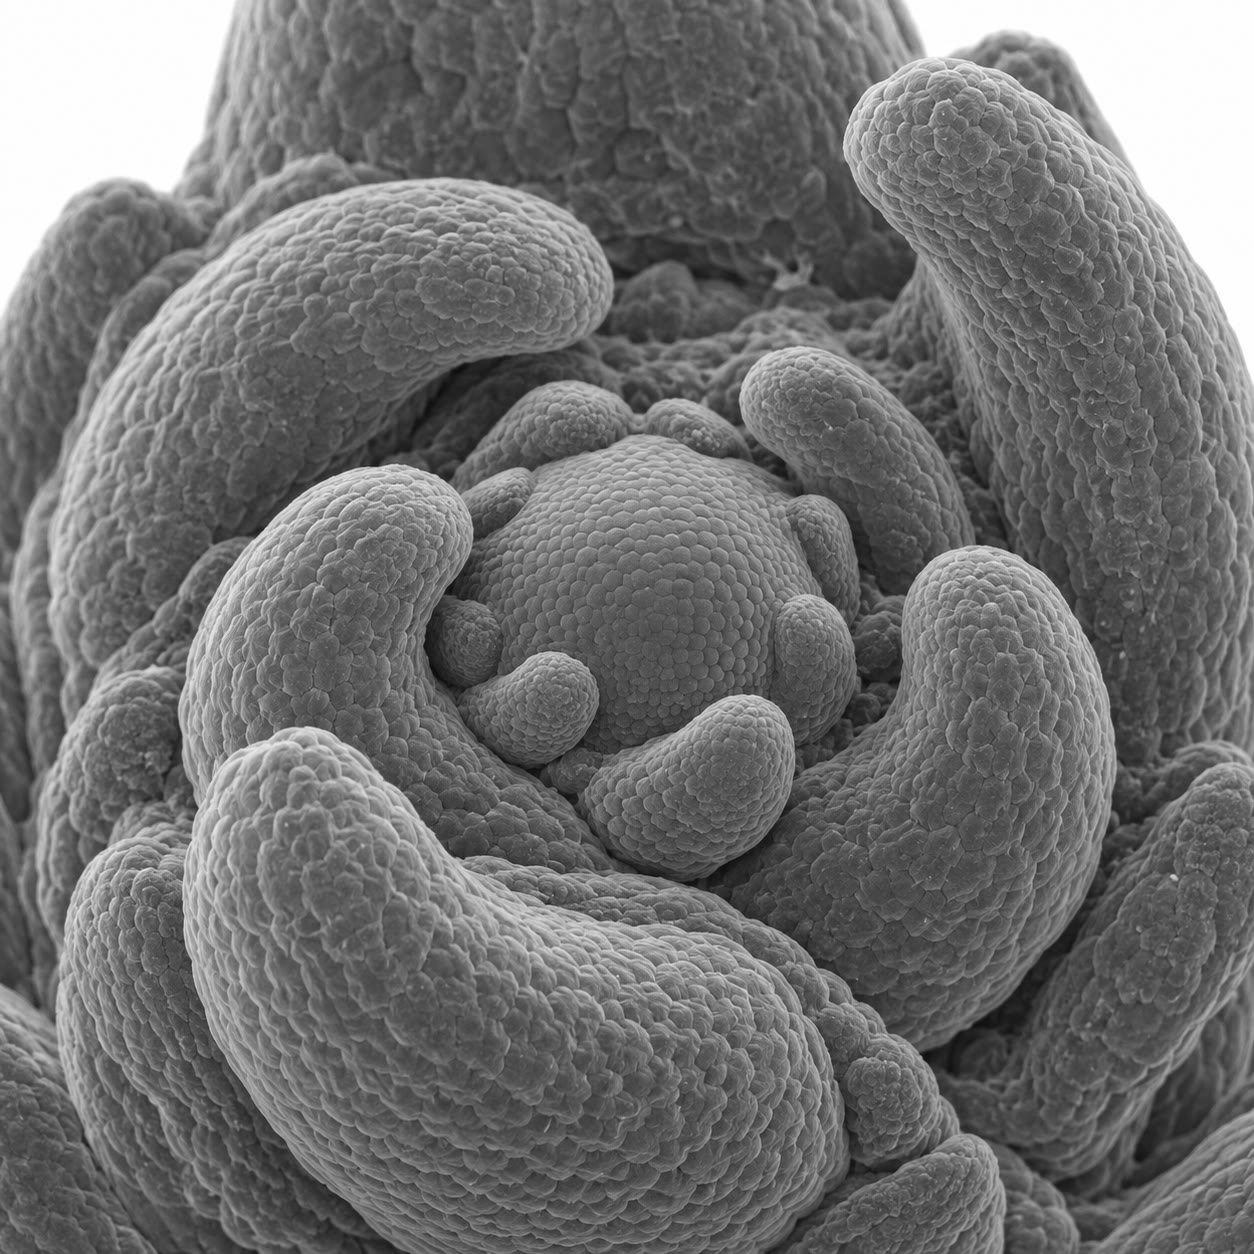
\includegraphics[width=0.44\linewidth]{images/book4/ai/b4-13-shoot-apex-sem.jpg}

{\small Un ápice caulinar al microscopio electrónico de barrido: la cúpula
lisa del \omterm{def:b2:plant-meristems:meristem}{meristemo} y la espiral de \omterm{prop:b2:plant-meristems:sam}{primordios foliares} a su alrededor,
cada uno nuevo situado en el hueco más amplio.}
\end{omfigure}

\begin{proposition}[Mantener las células madre: un bucle de retroalimentación]\label{prop:b2:plant-meristems:wus}
\index{WUSCHEL}\index{CLAVATA}\index{retroalimentación negativa!meristemo}
El tamaño de la reserva de \omterm{def:b2:cell-differentiation:differentiation}{células madre} se mantiene constante mediante
un bucle entre dos genes. Las células situadas justo debajo de la zona
central expresan el \omterm{prop:b2:cell-differentiation:transcriptional}{factor de transcripción} \emph{WUSCHEL} (WUS), cuyo
producto sube hacia las células superiores y las mantiene como \omterm{def:b2:cell-differentiation:differentiation}{células
madre}; las \omterm{def:b2:cell-differentiation:differentiation}{células madre}, a su vez, secretan un pequeño péptido,
\emph{CLAVATA3} (CLV3), que difunde hacia abajo, se une a un receptor
quinasa (CLV1) de las células que expresan WUS y reprime WUS. Más \omterm{def:b2:cell-differentiation:differentiation}{células
madre} significa más CLV3, menos WUS y menos \omterm{def:b2:cell-differentiation:differentiation}{células madre}; menos \omterm{def:b2:cell-differentiation:differentiation}{células
madre} significa menos CLV3, más WUS y más \omterm{def:b2:cell-differentiation:differentiation}{células madre}. La reserva es así
una magnitud regulada, como las gonadotropinas del
\cref{ch:b2:reproductive-hormones}, y la misma lógica --- una señal de la
población regulada que reprime el factor que la produce --- rige también
el \omterm{def:b2:plant-meristems:meristem}{meristemo} radicular.
\end{proposition}
\begin{proof}[Evidencia]
Los mutantes \emph{clavata} de Arabidopsis (Clark, Meyerowitz, década de
1990) tienen \omterm{def:b2:plant-meristems:meristem}{meristemos} que se hinchan hasta muchas veces su tamaño
normal, con hojas adicionales, órganos florales adicionales y tallos
fasciados (aplanados, en forma de cinta): el freno ha desaparecido. Los
mutantes \emph{wuschel} forman un \omterm{def:b2:plant-meristems:meristem}{meristemo} que se detiene tras unas pocas
hojas y después forma otros nuevos, cada uno de los cuales se detiene a su
vez: el acelerador ha desaparecido. En el doble mutante prevalece el
\omterm{def:b2:meiosis-heredity:vocabulary}{fenotipo} \emph{wuschel}, lo que sitúa WUS aguas abajo de CLV; y el péptido
CLV3 aplicado a un ápice silvestre reprime WUS en pocas horas.
\end{proof}

\begin{proposition}[El ápice radicular]\label{prop:b2:plant-meristems:ram}
\index{cofia}\index{centro quiescente}\index{zona de elongación}\index{pelo radicular}
Una raíz crece a partir de un \omterm{def:b2:plant-meristems:meristem}{meristemo} protegido detrás de una
\emph{cofia}, cuyas células se desprenden a medida que el extremo avanza
por el suelo y que secreta un mucílago lubricante y percibe la gravedad
(granos de almidón que sedimentan en sus células). En el centro del
\omterm{def:b2:plant-meristems:meristem}{meristemo}, un \emph{\omterm{prop:b2:plant-meristems:ram}{centro quiescente}} de unos pocos cientos de células
apenas se divide; mantiene como \omterm{def:b2:cell-differentiation:differentiation}{células madre} a las iniciales que lo
rodean --- de la cofia, la epidermis, la \omterm{def:b2:plant-meristems:wood}{corteza} y el cilindro vascular
---, igual que WUS mantiene las del tallo. Detrás del \omterm{def:b2:plant-meristems:meristem}{meristemo} viene la
\emph{\omterm{prop:b2:plant-meristems:ram}{zona de elongación}}, unos pocos milímetros en los que las células se
alargan de diez a veinte veces y empujan el extremo hacia delante;
después, la \emph{zona de \omterm{def:b2:cell-differentiation:differentiation}{diferenciación}}, donde la epidermis forma los
\emph{\omterm{prop:b2:plant-meristems:ram}{pelos radiculares}} y maduran el xilema y el floema. Las raíces
laterales no surgen en el extremo sino a partir del periciclo, en la
profundidad de la raíz madura, frente a los polos del xilema, y se abren
paso a través de la \omterm{def:b2:plant-meristems:wood}{corteza}. La auxina, fabricada en el tallo y
transportada hacia abajo, se acumula en el extremo y organiza toda la
disposición; el \omterm{prop:b2:plant-meristems:ram}{centro quiescente} se sitúa en su máximo.
\end{proposition}

\begin{omfigure}
\begin{tikzpicture}[every node/.style={font=\scriptsize}]
  % root outline
  \draw[thick, fill=omExo!10] (-1.0,4.5) -- (-1.0,0.6) .. controls (-1.0,-0.4) and (1.0,-0.4) .. (1.0,0.6) -- (1.0,4.5);
  % root cap
  \draw[thick, fill=omExo!45] (-0.9,0.8) .. controls (-1.1,-0.1) and (1.1,-0.1) .. (0.9,0.8) .. controls (0.5,0.4) and (-0.5,0.4) .. (-0.9,0.8);
  % meristem
  \fill[omThm!25] (-0.85,0.8) rectangle (0.85,1.7);
  \fill[omThm!70] (0,0.95) ellipse (0.25 and 0.12);
  % elongation zone
  \fill[omProp!20] (-0.85,1.7) rectangle (0.85,3.0);
  % differentiation zone with root hairs and vascular strand
  \fill[omDef!15] (-0.85,3.0) rectangle (0.85,4.5);
  \fill[omDef!50] (-0.15,3.0) rectangle (0.15,4.5);
  \foreach \y in {3.2,3.5,3.8,4.1,4.4} { \draw[omDef!80!black] (1.0,\y) -- (1.7,\y+0.1); \draw[omDef!80!black] (-1.0,\y) -- (-1.7,\y+0.1); }
  % lateral root primordium
  \draw[thick, fill=omThm!30] (0.15,4.0) .. controls (0.5,3.9) and (0.8,4.1) .. (0.9,4.3) .. controls (0.7,4.35) and (0.4,4.3) .. (0.15,4.3);
  % labels
  \draw (0.5,0.4) -- (2.2,0.2) node[right] {cofia};
  \draw (0.25,0.95) -- (2.2,0.9) node[right] {centro quiescente};
  \draw (0.85,1.4) -- (2.2,1.5) node[right] {meristemo (división)};
  \draw (0.85,2.4) -- (2.2,2.3) node[right, align=left] {zona de elongación:\\las células se alargan $10\times$};
  \draw (1.5,3.6) -- (2.2,3.4) node[right] {pelos radiculares};
  \draw (0.0,4.2) -- (2.2,4.2) node[right] {cilindro vascular};
  \draw (0.7,4.3) -- (2.2,4.9) node[right, align=left] {primordio de raíz lateral\\(del periciclo)};
  \draw[->, thick] (-2.4,4.5) -- (-2.4,0.6); \node[left, rotate=90, anchor=south] at (-2.5,2.5) {la auxina fluye hacia el extremo};
\end{tikzpicture}

{\small El ápice radicular: la cofia, el \omterm{def:b2:plant-meristems:meristem}{meristemo} con su \omterm{prop:b2:plant-meristems:ram}{centro
quiescente}, la \omterm{prop:b2:plant-meristems:ram}{zona de elongación} y la zona de \omterm{def:b2:cell-differentiation:differentiation}{diferenciación} con los
\omterm{prop:b2:plant-meristems:ram}{pelos radiculares} y los vasos maduros. Las raíces laterales nacen en la
profundidad, a partir del periciclo.}
\end{omfigure}

\begin{omfigure}
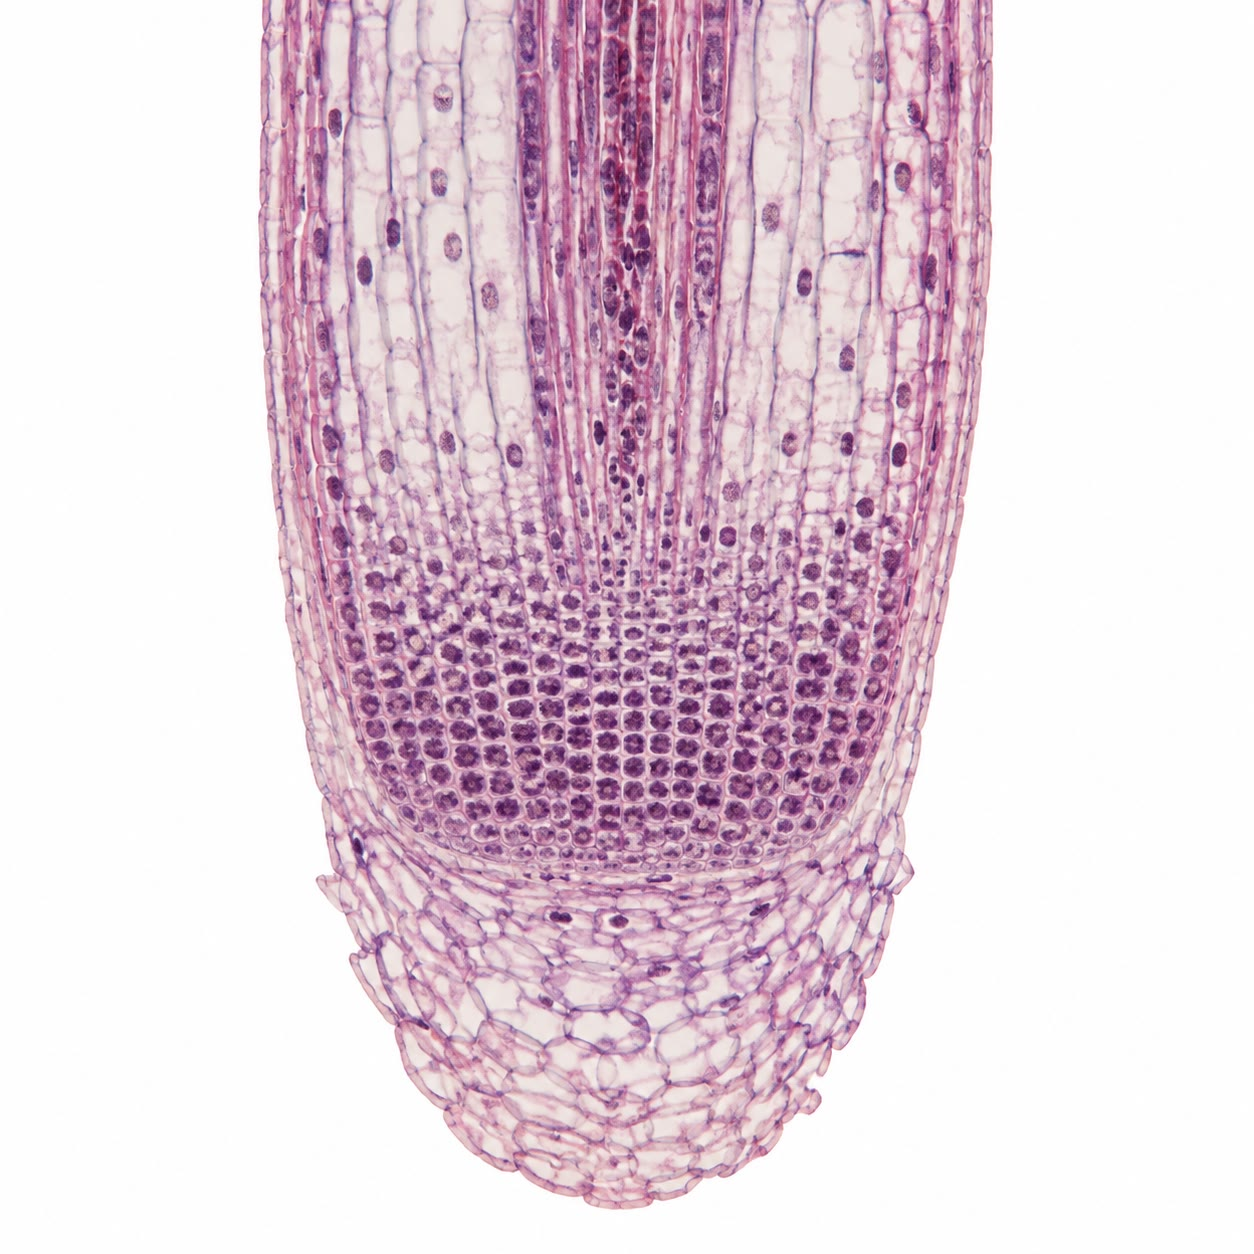
\includegraphics[width=0.42\linewidth]{images/book4/ai/b4-13-root-tip.jpg}

{\small Un ápice radicular en sección longitudinal: las células sueltas de
la cofia, el denso \omterm{def:b2:plant-meristems:meristem}{meristemo} con sus núcleos oscuros y las células que se
alargan por encima.}
\end{omfigure}

\section{Cómo crece una célula vegetal}

\begin{theorem}[La ecuación de Lockhart]\label{thm:b2:plant-meristems:lockhart}
\index{turgencia}\index{pared celular!extensibilidad}\index{ecuación de Lockhart}
Una célula vegetal crece estirando su pared bajo la presión de su propio
contenido. La pared solo cede de forma irreversible por encima de una
turgencia umbral $Y$, y entonces a un ritmo proporcional al exceso: la
tasa de crecimiento relativo de una célula de longitud $L$ es
\[
\frac{1}{L}\frac{\mathrm{d}L}{\mathrm{d}t} = \phi\,(P - Y) \quad (P > Y),
\]
donde $P$ es la presión de turgencia y $\phi$ la \emph{extensibilidad} de
la pared. El crecimiento se controla, por tanto, desde dos lados: desde el
agua, que fija $P$ (una célula marchita deja de crecer), y desde la pared,
que fija $\phi$ e $Y$ --- y es sobre la pared sobre la que actúan las
hormonas. La auxina hace que las células bombeen protones hacia la pared;
el ácido activa las \emph{expansinas}, proteínas que aflojan los enlaces
entre las fibrillas de celulosa y la matriz, lo que eleva $\phi$ y reduce
$Y$ en minutos (\emph{crecimiento ácido}). Con $\phi =
\qty{0.1}{h^{-1}.MPa^{-1}}$, $Y = \qty{0.3}{MPa}$ y $P =
\qty{0.6}{MPa}$, una célula se alarga un \qty{3}{\%} por hora y duplica su
longitud en un día; en la \omterm{prop:b2:plant-meristems:ram}{zona de elongación} de una raíz, donde las tasas
son varias veces mayores, una célula se alarga diez veces en unas pocas
horas.
\end{theorem}
\begin{proof}
La pared es un material viscoplástico: por debajo del límite de fluencia
se deforma elásticamente y se recupera; por encima, fluye a un ritmo
proporcional al exceso de tensión. La tensión en la pared es proporcional
a la presión de turgencia (para un cilindro de radio $r$ y espesor de
pared $w$, la tensión circunferencial es $Pr/w$), de modo que la velocidad
de deformación plástica es proporcional a $P - Y$ con una constante $\phi$
que engloba la geometría y las propiedades del material de la pared. La
velocidad de deformación es, por definición,
$(1/L)\,\mathrm{d}L/\mathrm{d}t$. Numéricamente,
$0.1\times(0.6 - 0.3) = \qty{0.03}{h^{-1}}$, y $L$ se duplica cuando
$0.03\,t = \ln 2$, $t = \qty{23}{h}$.
\end{proof}

\begin{omfigure}
\begin{tikzpicture}
\begin{axis}[
  width=0.7\linewidth, height=5.4cm,
  axis x line=bottom, axis y line=left,
  xmin=0, xmax=1.0, ymin=0, ymax=0.09,
  xlabel={presión de turgencia $P$ (\unit{MPa})}, ylabel={tasa de crecimiento relativo (\unit{h^{-1}})},
  xlabel style={font=\small, at={(axis description cs:0.5,-0.13)}, anchor=north},
  ylabel style={font=\small},
  tick label style={font=\small}, xtick={0,0.3,0.6,0.9}, ytick={0,0.03,0.06,0.09},
  yticklabels={0,0.03,0.06,0.09}, scaled y ticks=false,
  legend style={font=\scriptsize, at={(0.03,0.97)}, anchor=north west, draw=none},
  clip=false,
]
\addplot[very thick, omDef, domain=0:0.3, samples=2, forget plot] {0};
\addplot[very thick, omDef, domain=0.3:1.0, samples=2] {0.1*(x-0.3)};
\addlegendentry{$\phi = 0.1$, $Y = 0.3$}
\addplot[very thick, omThm, domain=0:0.2, samples=2, forget plot] {0};
\addplot[very thick, omThm, domain=0.2:0.65, samples=2] {0.2*(x-0.2)};
\addlegendentry{con auxina: $\phi = 0.2$, $Y = 0.2$}
\draw[dashed, gray] (axis cs:0.6,0) -- (axis cs:0.6,0.03); \node[font=\scriptsize, anchor=west] at (axis cs:0.61,0.015) {$P$ típica};
\end{axis}
\end{tikzpicture}

{\small La ley de Lockhart: no hay crecimiento por debajo de la turgencia
umbral, y por encima el ritmo es proporcional al exceso. La auxina, al
aflojar la pared, reduce el umbral y aumenta la pendiente de la recta, y a
la misma turgencia la célula crece varias veces más deprisa.}
\end{omfigure}

\begin{example}[De dónde viene el agua]\label{ex:b2:plant-meristems:water}
A medida que la pared cede, la turgencia caería y el crecimiento se
detendría si no entrara agua al mismo ritmo: la célula en crecimiento es
una fuga que se rellena sola. El agua procede del xilema, a favor de un
pequeño gradiente de potencial hídrico, y su ritmo de entrada lo fija la
conductancia hidráulica de la membrana; el crecimiento es más rápido de
noche, cuando la transpiración es baja y la turgencia alta, y una hoja de
maíz puede alargarse \qty{10}{cm} entre el anochecer y el amanecer. Con
sequía, las células fabrican solutos (\emph{ajuste osmótico}) para
mantener $P$ por encima de $Y$, y cuando eso falla la hoja deja de crecer
días antes de marchitarse.
\end{example}

\section{Las hormonas y la forma del tallo}

\begin{proposition}[La auxina y la dominancia apical]\label{prop:b2:plant-meristems:apical}
\index{auxina}\index{dominancia apical}\index{transporte polar de la auxina}\index{citoquinina}
La \emph{auxina} (ácido indol-3-acético) se fabrica en el ápice del tallo y
en las hojas jóvenes y se transporta tallo abajo, de célula en célula, a
alrededor de \qty{1}{cm/h}, mediante proteínas transportadoras (PIN)
situadas en el extremo inferior de cada célula --- un \emph{transporte
polar} que da a la planta un eje de arriba abajo. La corriente de auxina
que desciende del ápice mantiene latentes las yemas axilares situadas por
debajo (\emph{\omterm{prop:b2:plant-meristems:apical}{dominancia apical}}), en parte impidiéndoles exportar su
propia auxina al tallo y en parte induciendo estrigolactonas y
reprimiendo la citoquinina. Si se corta el ápice, las yemas más cercanas
al corte brotan en pocos días y la planta se vuelve frondosa --- que es lo
que aprovechan la poda y el despunte. Las \emph{citoquininas}, fabricadas
en los ápices radiculares y transportadas hacia arriba por el xilema,
favorecen el brote de las yemas y la división celular; las
\emph{giberelinas} alargan los entrenudos (los guisantes enanos y el trigo
semienano de la Revolución Verde tienen defectos en su síntesis o en su
percepción); el ácido abscísico y el etileno frenan el crecimiento en
condiciones de estrés. La forma del tallo --- alto o frondoso, erguido o
extendido --- es una negociación entre estas señales, y el equilibrio
entre raíz y tallo lo fija la auxina que baja frente a la citoquinina que
sube.
\end{proposition}
\begin{proof}[Evidencia]
Thimann y Skoog (1934) cortaron el ápice de plantas de judía: las yemas
laterales crecieron. Un bloque de agar con auxina, colocado sobre el
muñón cortado, las mantuvo latentes igual que el ápice; el agar solo no.
Went (1928) ya había medido la auxina por la curvatura que producía en
coleóptilos decapitados de avena al colocarla a un lado del muñón --- el
primer bioensayo de una hormona vegetal, y el origen del nombre, del
griego ``crecer''. La polaridad del transporte se demostró colocando agar
con auxina en un extremo de un segmento de tallo y encontrándola en un
bloque receptor del otro extremo solo cuando el segmento estaba orientado
con el ápice hacia arriba, cualquiera que fuese la orientación del
segmento en el campo de la gravedad.
\end{proof}

\begin{omfigure}
\begin{tikzpicture}[every node/.style={font=\scriptsize}, >=stealth]
  \foreach \x/\lab/\apex/\aux in {0/{intacta: con ápice,\\yemas latentes}/1/0, 4.2/{decapitada:\\las yemas brotan}/0/0, 8.4/{decapitada + auxina\\en el muñón: latentes}/0/1} {
    \begin{scope}[xshift=\x cm]
      \draw[very thick, omExo!70!black] (0,0) -- (0,3.4);
      \foreach \y in {0.8,1.6,2.4} { \draw[thick, omExo!70!black] (0,\y) -- (-0.8,\y+0.4); \draw[thick, omExo!70!black] (0,\y+0.4) -- (0.8,\y+0.8); }
      \ifnum\apex=1 \draw[thick, fill=omThm!40] (0,3.5) ellipse (0.25 and 0.3); \draw[->, thick, omThm] (0.35,3.2) -- (0.35,1.0); \node[omThm, right] at (0.4,2.1) {auxina}; \fi
      \ifnum\apex=0 \draw[thick] (-0.3,3.4) -- (0.3,3.4); \fi
      \ifnum\aux=1 \draw[thick, fill=omThm!40] (-0.25,3.4) rectangle (0.25,3.75); \node[omThm, right] at (0.3,3.6) {agar con auxina}; \draw[->, thick, omThm] (0.35,3.2) -- (0.35,1.0); \fi
      \ifnum\apex=1 \foreach \y in {0.8,1.6,2.4} \fill[gray!60] (-0.12,\y+0.1) circle (0.08); \fi
      \ifnum\aux=1 \foreach \y in {0.8,1.6,2.4} \fill[gray!60] (-0.12,\y+0.1) circle (0.08); \fi
      \ifnum\apex=0 \ifnum\aux=0 \foreach \y in {0.8,1.6,2.4} { \draw[thick, omExo!70!black] (-0.1,\y+0.1) -- (-0.7,\y+0.9); \draw[thick, omExo!70!black] (-0.7,\y+0.9) -- (-1.0,\y+1.1); \draw[thick, omExo!70!black] (-0.7,\y+0.9) -- (-0.75,\y+1.25); } \fi\fi
      \node[below, align=center] at (0,-0.3) {\lab};
    \end{scope}
  }
\end{tikzpicture}

{\small La \omterm{prop:b2:plant-meristems:apical}{dominancia apical}: el experimento de Thimann y Skoog. El ápice
mantiene latentes las yemas axilares; eliminarlo las libera; la auxina
sobre el muñón cortado sustituye al ápice.}
\end{omfigure}

\begin{example}[Señal rápida, molécula lenta]\label{ex:b2:plant-meristems:transport}
El transporte polar desplaza la auxina \qty{1}{cm} en una hora; la difusión
sola tardaría, para el mismo centímetro, $t = x^2/2D = 10^{-4}/(2\times
10^{-9}) = \qty{5e4}{s}$ --- catorce horas ---, y para los diez centímetros
hasta una yema inferior, sesenta días. El sistema de bombeo y relevo de los
transportadores PIN es lo que hace utilizable una señal hormonal a lo
largo de una planta; esos mismos transportadores, desplazados hacia el lado
sombreado de un tallo, lo curvan hacia la luz
(\cref{ch:b2:plant-plasticity}).
\end{example}

\section{El crecimiento secundario: madera y corteza}

\begin{definition}[El cámbium vascular y la madera]\label{def:b2:plant-meristems:wood}
\index{cámbium vascular}\index{madera}\index{anillo anual}\index{corteza}\index{peridermis}
En un tallo leñoso, los haces de xilema y de floema primarios se unen,
durante el primer año, en un cilindro continuo de células en división, el
\emph{\omterm{def:b2:plant-meristems:meristem}{cámbium} vascular}. Sus células se dividen tangencialmente y añaden
\emph{xilema secundario} --- \emph{madera} --- hacia dentro y
\emph{floema secundario} hacia fuera, de modo que el \omterm{def:b2:plant-meristems:meristem}{cámbium} se desplaza
hacia fuera a medida que el tronco se engrosa, y añaden de vez en cuando
divisiones radiales para ampliar el anillo. En los climas estacionales, la
madera formada en primavera tiene vasos anchos y de pared delgada
(\emph{madera temprana}) y la de verano, vasos estrechos y de pared gruesa
(\emph{madera tardía}), de modo que cada año deja un \emph{anillo anual}
visible; los anillos registran la edad del árbol y, en su anchura, el
clima de cada año (dendrocronología). Solo los anillos externos, la
\emph{albura}, conducen; los internos, el \emph{duramen}, están muertos,
obstruidos y oscurecidos por resinas y taninos, y sirven de esqueleto al
árbol. Por fuera del floema, un segundo \omterm{def:b2:plant-meristems:meristem}{meristemo} lateral, el
\emph{felógeno}, forma la \emph{peridermis} --- capas de células de corcho,
muertas e impermeabilizadas con suberina ---, que con el floema antiguo
constituye la \emph{corteza}. Un tronco es así una fina envoltura viva de
\omterm{def:b2:plant-meristems:meristem}{cámbium}, albura y floema alrededor de un núcleo muerto, bajo una piel
muerta.
\end{definition}

\begin{omfigure}
\begin{tikzpicture}[every node/.style={font=\scriptsize}]
  \fill[omExo!60] (0,0) circle (3.0);
  \fill[omDef!20] (0,0) circle (2.75);
  \fill[omDef!35] (0,0) circle (2.2);
  \foreach \r in {0.4,0.7,1.0,1.3,1.6,1.9,2.2} \draw[omDef!80!black, thin] (0,0) circle (\r);
  \fill[omExo!80!black] (0,0) circle (1.3);
  \foreach \r in {0.4,0.7,1.0} \draw[omExo!40, thin] (0,0) circle (\r);
  \draw[very thick, omThm] (0,0) circle (2.5);
  \draw (2.9,0.6) -- (3.9,1.6) node[right, align=left] {corteza: corcho (peridermis)\\y floema antiguo};
  \draw (2.62,0.0) -- (3.9,0.6) node[right] {floema secundario, vivo};
  \draw (2.5,-0.4) -- (3.9,-0.4) node[right] {cámbium vascular (rojo)};
  \draw (1.9,-1.1) -- (3.9,-1.4) node[right, align=left] {albura: anillos recientes,\\conductores};
  \draw (0.5,-0.9) -- (3.9,-2.4) node[right, align=left] {duramen: anillos antiguos,\\muertos, obstruidos};
  \draw (-1.7,1.5) -- (-3.6,2.4) node[left, align=right] {un anillo anual:\\madera temprana clara,\\madera tardía oscura};
\end{tikzpicture}

{\small Un tronco en sección transversal. El \omterm{def:b2:plant-meristems:meristem}{cámbium} (rojo) añade cada año
\omterm{def:b2:plant-meristems:wood}{madera} hacia dentro y floema hacia fuera; los anillos recientes conducen,
los antiguos forman el duramen muerto; el corcho y el floema antiguo
forman la \omterm{def:b2:plant-meristems:wood}{corteza}.}
\end{omfigure}

\begin{theorem}[Por qué un árbol viejo añade más madera]\label{thm:b2:plant-meristems:rings}
Un tronco de radio $r$ y altura $h$ cuyo \omterm{def:b2:plant-meristems:meristem}{cámbium} añade cada año un anillo
de espesor $\Delta r$ gana un volumen de \omterm{def:b2:plant-meristems:wood}{madera}
\[
\Delta V \approx 2\pi r\,h\,\Delta r
\]
al año: con una anchura de anillo constante, el incremento anual crece en
proporción al radio, y un árbol de \qty{50}{cm} de radio añade diez veces
la \omterm{def:b2:plant-meristems:wood}{madera} de uno de \qty{5}{cm}, aunque sus anillos no sean más anchos. Un
tronco de \qty{25}{cm} de radio y \qty{10}{m} de altura que añade
\qty{4}{mm} al año gana \qty{0.063}{m^3}, unos \qty{30}{kg} de \omterm{def:b2:plant-meristems:wood}{madera}
seca --- \qty{15}{kg} de carbono, tomados del aire por la copa en una sola
estación.
\end{theorem}
\begin{proof}
La \omterm{def:b2:plant-meristems:wood}{madera} añadida es una envoltura cilíndrica de circunferencia $2\pi r$,
espesor $\Delta r$ y altura $h$; su volumen es $2\pi r h\Delta r$
a primer orden en $\Delta r$ (exactamente $\pi h[(r + \Delta r)^2 - r^2]
= \pi h(2r\Delta r + \Delta r^2)$). Con $r = 0.25$, $h = 10$,
$\Delta r = 0.004$: $2\pi\times 0.25\times 10\times 0.004 =
\qty{0.063}{m^3}$; a \qty{500}{kg/m^3} en seco, \qty{31}{kg}, la mitad de
ellos carbono.
\end{proof}

\begin{omfigure}
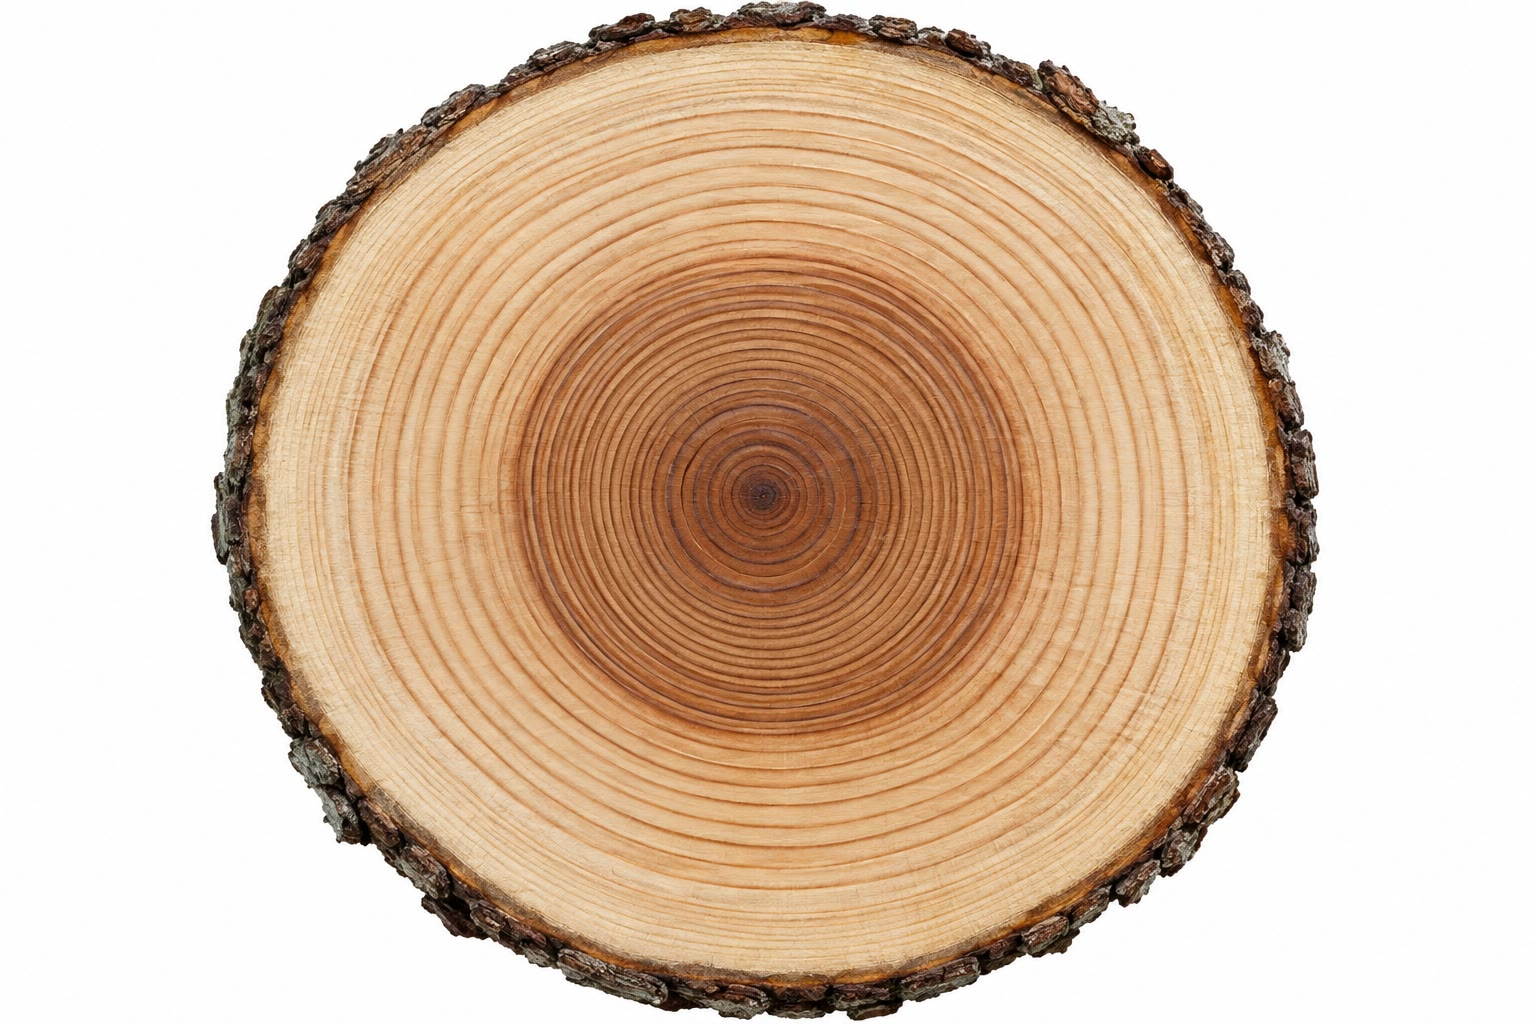
\includegraphics[width=0.5\linewidth]{images/book4/ai/b4-13-wood-rings.jpg}

{\small Un tronco de pino en sección transversal: los \omterm{def:b2:plant-meristems:wood}{anillos anuales},
cada uno con una banda clara de \omterm{def:b2:plant-meristems:wood}{madera} temprana y otra oscura de \omterm{def:b2:plant-meristems:wood}{madera}
tardía, el duramen más oscuro y la \omterm{def:b2:plant-meristems:wood}{corteza}.}
\end{omfigure}

\section{Ejercicios}

\begin{exercise}[$\star$]\label{exo:b2:plant-meristems:1}
Defínase \omterm{def:b2:plant-meristems:meristem}{meristemo}, y nómbrense los cuatro \omterm{def:b2:plant-meristems:meristem}{meristemos} de una planta leñosa
con lo que produce cada uno.
\end{exercise}

\begin{exercise}[$\star$]\label{exo:b2:plant-meristems:2}
Enumérense las zonas de un ápice radicular desde la cofia hacia arriba,
con lo que le ocurre a una célula en cada una. ¿De dónde proceden las
raíces laterales?
\end{exercise}

\begin{exercise}[$\star$]\label{exo:b2:plant-meristems:3}
Descríbanse el experimento de Thimann y Skoog, su control y su conclusión.
\end{exercise}

\begin{exercise}[$\star$]\label{exo:b2:plant-meristems:4}
Una sección de tronco muestra 60 anillos, los 15 externos claros y el
resto oscuros. Dense la edad del árbol y la edad de su albura, y dígase
qué parte del tronco está viva.
\end{exercise}

\begin{exercise}[$\star\star$]\label{exo:b2:plant-meristems:5}
Con $\phi = \qty{0.1}{h^{-1}.MPa^{-1}}$ e $Y = \qty{0.3}{MPa}$, calcúlense
la tasa de crecimiento relativo a $P = 0.4$, $0.6$ y \qty{0.8}{MPa}, y el
tiempo de duplicación en cada caso. Una sequía reduce $P$ a
\qty{0.25}{MPa}: ¿qué ocurre?
\end{exercise}

\begin{exercise}[$\star\star$]\label{exo:b2:plant-meristems:6}
Las hojas sucesivas surgen a \qty{137.5}{\degree} unas de otras.
Calcúlense las posiciones angulares de las hojas 1 a 8 (módulo
\qty{360}{\degree}) y muéstrese que ningún par de las ocho primeras está a
menos de \qty{20}{\degree}. ¿Por qué le importa esto a la planta?
\end{exercise}

\begin{exercise}[$\star\star$]\label{exo:b2:plant-meristems:7}
Un árbol de \qty{12}{m} de altura añade anillos de \qty{3}{mm}. Calcúlense
la \omterm{def:b2:plant-meristems:wood}{madera} añadida el año en que su radio es de \qty{5}{cm} y el año en que
es de \qty{40}{cm}, y el carbono correspondiente (densidad en seco de
\qty{500}{kg/m^3}, la mitad carbono).
\end{exercise}

\begin{exercise}[$\star\star$]\label{exo:b2:plant-meristems:8}
Predíganse los \omterm{def:b2:meiosis-heredity:vocabulary}{fenotipos} de un mutante \emph{clv3}, de un mutante
\emph{wus} y del doble mutante, y explíquese a partir del doble mutante el
orden de los dos genes en el bucle.
\end{exercise}

\begin{exercise}[$\star\star$]\label{exo:b2:plant-meristems:9}
La auxina se transporta a \qty{1}{cm/h}; su coeficiente de difusión en el
tejido es de \qty{1e-9}{m^2/s}. ¿Cuánto tarda la señal en llegar a una yema
situada \qty{20}{cm} por debajo del ápice por transporte, y por difusión
($t = x^2/2D$)? ¿Qué le aporta a la planta el transporte polar?
\end{exercise}

\begin{exercise}[$\star\star\star$]\label{exo:b2:plant-meristems:10}
Una raíz de maíz crece \qty{3}{cm} al día. Las células del \omterm{def:b2:plant-meristems:meristem}{meristemo} miden
\qty{20}{\micro m} de largo y se alargan diez veces antes de madurar; cada
fila celular tiene unas \num{100} células en división. ¿Cuántas células
debe producir al día el \omterm{def:b2:plant-meristems:meristem}{meristemo} de cada fila, y qué duración del ciclo
celular implica eso?
\end{exercise}

\begin{exercise}[$\star\star\star$]\label{exo:b2:plant-meristems:11}
Los trigos semienanos de la década de 1960 llevan \omterm{def:b2:genome-diversification:mutation}{mutaciones} que hacen la
planta insensible a la giberelina. Explíquese por qué son bajos, por qué
una planta baja puede rendir más grano cuando se abona intensamente, y por
qué la misma \omterm{def:b2:genome-diversification:mutation}{mutación} sería una desventaja en una planta silvestre.
\end{exercise}

\begin{exercise}[$\star\star\star$]\label{exo:b2:plant-meristems:12}
``Un animal se construye una vez; una planta se construye durante toda su
vida.'' Discútanse las consecuencias del crecimiento meristemático para la
capacidad de una planta de responder a su entorno, de sobrevivir a los
daños y de vivir milenios --- y un coste de esta estrategia.
\end{exercise}

\section{Problema: un árbol en cifras}

\begin{problem}[{Problema de fin de semana --- se sigue un árbol joven
durante un año: las hojas que forma su ápice, el crecimiento de un
entrenudo según la ley de Lockhart, la madera que produce su cámbium y el
carbono que cuesta, y la respuesta de sus yemas a la poda, hasta llegar a
las hojas por año, el crecimiento horario del entrenudo y la madera del
año}]
\label{pb:b2:plant-meristems:1}
Un tilo joven tiene \num{200} ápices caulinares en crecimiento; cada ápice
inicia una hoja cada \num{3} días durante una estación de \num{150} días, a
intervalos de \qty{137.5}{\degree}. Un entrenudo en crecimiento mide
\qty{2}{cm}, y sus células tienen $\phi = \qty{0.05}{h^{-1}.MPa^{-1}}$, $Y =
\qty{0.35}{MPa}$; la turgencia es de \qty{0.55}{MPa} de día y de
\qty{0.75}{MPa} de noche (\qty{12}{h} cada una). El tronco mide
\qty{8}{m} de altura y tiene un radio de \qty{10}{cm}; el \omterm{def:b2:plant-meristems:meristem}{cámbium} añade
\qty{5}{mm} al año; la \omterm{def:b2:plant-meristems:wood}{madera} seca tiene \qty{500}{kg/m^3} y es carbono en
su mitad. La copa lleva \qty{80}{m^2} de hojas que fijan en neto \qty{4}{g}
de carbono por metro cuadrado al día durante \num{150} días.

\medskip
\noindent\textbf{Parte I --- Las hojas.}
\begin{enumerate}
  \item ¿Cuántas hojas forma un ápice en una estación? ¿Y todo el árbol?
  \item Calcúlense las posiciones angulares de las hojas 1 a 5 de un tallo.
  \item ¿Al cabo de cuántas hojas cae una hoja a menos de
        \qty{10}{\degree} de la hoja 1? (Pruébense múltiplos de
        \qty{137.5}{\degree}.)
  \item ¿Qué consigue el ángulo áureo para la planta, y qué transporte
        hormonal lo produce?
  \item Si cada hoja tiene una superficie de \qty{80}{cm^2}, ¿qué superficie
        foliar construye el árbol en una estación? Compárese con los
        \qty{80}{m^2} que lleva en pleno verano.
  \item El árbol es caducifolio. ¿Qué fracción de su superficie foliar
        reconstruye cada primavera, y de dónde procede el carbono de las
        primeras hojas?
  \item Una \omterm{def:b2:genome-diversification:mutation}{mutación} \emph{clv3} triplica el tamaño de cada ápice. ¿Qué
        cambiaría en las respuestas a las preguntas 1 y 5, y qué aspecto
        tendrían los tallos?
\end{enumerate}

\medskip
\noindent\textbf{Parte II --- Un entrenudo.}
\begin{enumerate}[resume]
  \item Calcúlese la tasa de crecimiento relativo de día y de noche.
  \item Calcúlese la longitud añadida en un día y en una noche, partiendo de
        \qty{2}{cm}.
  \item Al cabo de cuatro días así, ¿qué longitud tiene el entrenudo?
        (Trátese el crecimiento como compuesto, $L(t) = L_0 e^{rt}$ con la
        tasa media.)
  \item Un tratamiento con giberelina reduce $Y$ a \qty{0.25}{MPa}.
        Vuélvanse a calcular las tasas de día y de noche.
  \item Una sequía mantiene la turgencia en \qty{0.4}{MPa} de día y de
        noche. Calcúlese la tasa, y dígase qué hace el ajuste osmótico.
  \item Explíquese por qué el crecimiento nocturno supera al diurno aunque
        la fotosíntesis se produce de día.
\end{enumerate}

\medskip
\noindent\textbf{Parte III --- La \omterm{def:b2:plant-meristems:wood}{madera}.}
\begin{enumerate}[resume]
  \item Calcúlense el volumen de \omterm{def:b2:plant-meristems:wood}{madera} añadido este año y su masa seca.
  \item Calcúlese el carbono que contiene.
  \item Calcúlese el carbono fijado por la copa a lo largo de la estación.
  \item ¿Qué fracción del carbono de la copa se destinó a la \omterm{def:b2:plant-meristems:wood}{madera} del
        tronco? Nómbrense otros tres sumideros.
  \item Dentro de veinte años, con la misma anchura de anillo, ¿cuál será
        el incremento anual de \omterm{def:b2:plant-meristems:wood}{madera}? ¿Por qué aumenta?
  \item Dos anillos del tronco tienen la mitad de anchura que sus vecinos.
        Propónganse dos causas y cómo las distinguiría un
        dendrocronólogo.
\end{enumerate}

\medskip
\noindent\textbf{Parte IV --- Yemas y poda.}
\begin{enumerate}[resume]
  \item El jardinero despunta todos los ápices. Predíganse la respuesta de
        las yemas axilares y la forma del árbol al cabo de un mes.
  \item ¿Cómo alteraría la respuesta una pasta de auxina en cada corte?
  \item Un seto se recorta seis veces al año. Explíquese, con la \omterm{prop:b2:plant-meristems:apical}{dominancia
        apical}, por qué se vuelve denso.
  \item Un árbol talado a ras de tocón vuelve a crecer con una docena de
        brotes. ¿De dónde proceden, y por qué una planta puede sobrevivir a
        la pérdida de todos sus tallos cuando un animal no sobrevive a la
        pérdida de su cabeza?
  \item La citoquinina de las raíces aumenta tras regar las raíces.
        Predígase el efecto sobre el brote de las yemas.
  \item Enúnciese el resultado: hojas por ápice y por árbol en una
        estación, las tasas de crecimiento diurna y nocturna del entrenudo,
        y la \omterm{def:b2:plant-meristems:wood}{madera} y el carbono del año.
\end{enumerate}
\end{problem}
